\subsection{Критерий <<трёх сигм>>. Расстояние Махаланобиса}

Для начала рассмотрим классический и основополагающий метод обнаружения аномалий с использованием критерия <<трех сигм>>. Этот метод является статистическим и основывается на предположении, что данные распределены нормально, и аномалии могут быть выявлены как те, которые выходят за пределы трех среднеквадратичных отклонений от среднего значения. Из простоты метода следуют очевидные ограничения на область его применения: при значительном отклонении данных от распределения Гаусса эффективность и точность метода может значительно снизиться. Для использования критерия необходимо рассчитать среднее значение и стандартное отклонение по формулам (\ref{average}) и (\ref{standard_deviation}) соответственно.

\begin{equation}\label{average}
    \mu = \frac{1}{n} \sum\limits_{i = 1}^{n}x_i,
\end{equation}

\begin{equation}\label{standard_deviation}
    \sigma = \sqrt{\frac{1}{n} \sum\limits_{i = 1}^{n}(x_i - \mu)^2},
\end{equation}
где $n$ – количество элементов выборки, \\
$x_i$ --- $i$-ый элемент выборки.

Затем аномалии определяются как те значения, которые находятся за пределами интервала, определенного трех среднеквадратичных отклонений от среднего (см. рисунок~\ref{fig:three-sigma}).

\begin{figure}
  \centering
  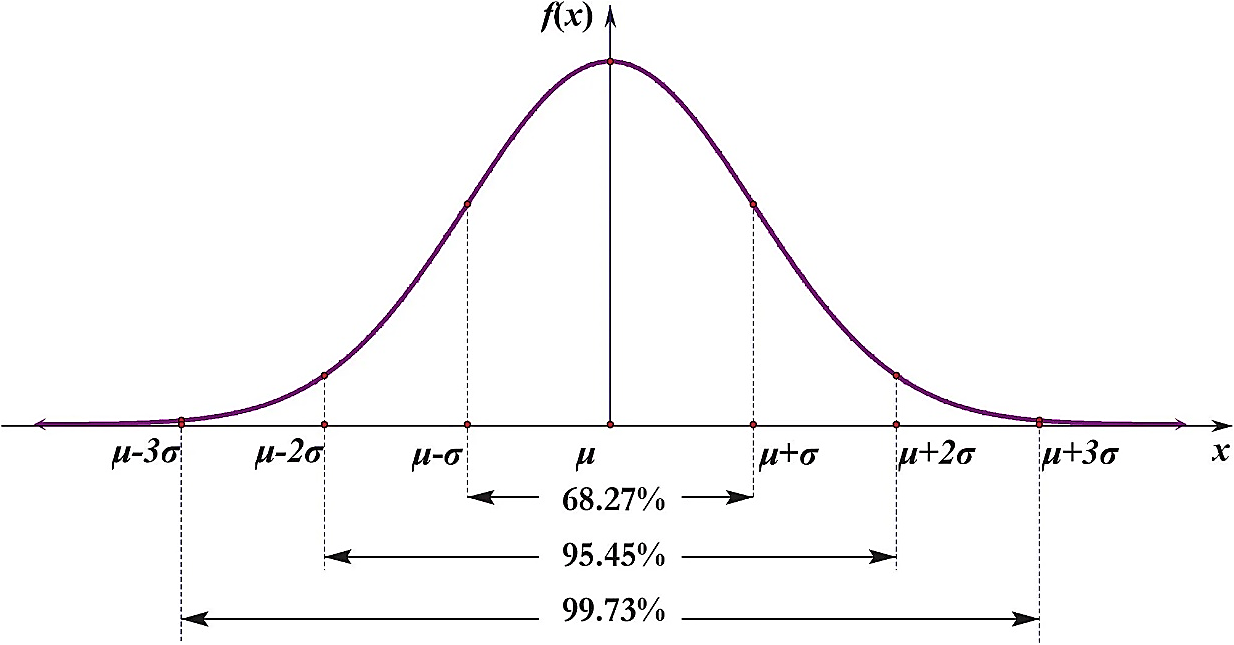
\includegraphics[scale=0.25]{inc/images/three-sigma.png}
  \caption{График нормального распределения и процент попадания в отрезки, равные среднеквадратичному отклонению \cite{Three-Sigma-Limits}}
  \label{fig:three-sigma}
\end{figure}

Помимо своей простоты, данный метод имеет ограничения в эффективности при обнаружении сложных нелинейных закономерностей в данных. Однако в многомерном случае признаки могут коррелировать между собой, что исключает прямое применение данного подхода. Для учета ковариационной структуры признаков вводится квадрат расстояния Махаланобиса, заданный соотношением (\ref{D_M_2}).

\begin{equation}\label{D_M_2}
D_M^2(\overline{x}_i) = (\overline{x}_i - \overline{\mu})^T S^{-1} (\overline{x}_i - \overline{\mu}),
\end{equation}
где $\overline{\mu}$ --- \textit{вектор} средних значений соответствующих признаков, \\
$S$  --- ковариационная матрица.

Функция принятия решения в многомерном случае принимает вид (\ref{f_3sigma_maha}):
\begin{equation}\label{f_3sigma_maha}
    f(\overline{x}_i) = \begin{cases}
         \ \ 1, & \text{если } D_M(\overline{x}_i) > r, \\
        -1, & \text{иначе},
    \end{cases}
\end{equation}
где порог $r$ подбирается так, чтобы вероятность ложноположительного срабатывания (ошибка I рода) не превышала заданное значение.

При условии, что вектор признаков \(\overline{x}_i\) распределён нормально, величина \(D_M^2(\overline{x}_i)\) следует распределению \(\chi^2_d\) с \(d\) степенями свободы (где \(d\) --- размерность вектора признаков), порог \(r\) можно определить из равенства (\ref{r_equation}).

\begin{equation}\label{r_equation}
    P\Big\{ \chi^2_d > r^2 \Big\} = p
\end{equation}

Тогда вероятности ошибок I-го и II-го рода определяются соотношениями (\ref{alpha_3sigma}) и (\ref{beta_3sigma}) соответственно.
\begin{equation}\label{alpha_3sigma}
\alpha = P\Big\{ D_M(\overline{x}_i) > r \ \Big|\ t_i\ -\ \text{«нормальный» экземпляр} \Big\}.
\end{equation}

\begin{equation}\label{beta_3sigma}
    \beta = P\Big\{ D_M(\overline{x}_i) \le r \ \Big|\ t_i\ -\ \text{«аномальный» экземпляр} \Big\}.
\end{equation}

Таким образом, метод позволяет установить строгие границы для функции принятия решения $f$. При условии нормальности распределения данных, критерий обеспечивает очень малую вероятность ошибки I-го рода, что удовлетворяет ограничению, заданному в постановке задачи, и позволяет эффективно минимизировать $\beta$, что соответствует цели оптимизации, сформулированной в (\ref{task_formulation}). Однако сетевой трафик редко может быть описан распределением Гаусса, ввиду нерегулярности событий в вычислительных сетях, что даёт повод для рассмотрения других путей решения задачи. Кроме того, такой подход не учитывает структуру данных и контекст анализа. Однако он включён рассмотрение ввиду его первоначальной каноничности для решения поставленной задачи. Многие статистические модели используют, развивают и усовершенствуют данный подход.
